\section{排序}
排序算法将列表的数据元素按一定的顺序排列。 排序是现代数据和信息服务的基础,因为如果数据集顺序正确,
则可以显着降低从数据集中检索信息的计算复杂性。 例如,排序通常用于规范化数据,以便在数据列表之间进行快速比较和协调。 
此外,如果数据按一定顺序排列,则可以提高许多数据处理算法的效率。 
由于其重要性,高效排序算法一直是许多计算机科学研究的主题。 
即使使用这些高效的算法,对大型数据列表进行排序仍然很耗时,并且可以从并行执行中受益。 
并行化高效排序算法具有挑战性,需要精心设计。 本章介绍两种重要的高效排序算法的并行设计:基数排序和合并排序。 
本章的大部分内容致力于基数排序; 基于第 12 章“合并”中介绍的并行合并模式,简要讨论了合并排序。 
还简要讨论了其他流行的并行排序算法,例如转置排序和采样排序。

\subsection{背景}
排序是计算机最早的应用之一。 排序算法将列表的元素按一定顺序排列。 排序算法强制执行的顺序取决于这些元素的性质。 
流行顺序的示例是数字的数字顺序和文本字符串的字典顺序。 更正式地说,任何排序算法都必须满足以下两个条件:
\begin{enumerate}
   \item 输出按非递减或非递增顺序排列。 对于非降序,根据所需的顺序,每个元素不小于前一个元素。 
   		对于非递增顺序,根据所需的顺序,每个元素不大于前一个元素。

   \item 输出是输入的排列。 也就是说,算法必须保留所有原始输入元素,同时将它们重新排序到输出中。
\end{enumerate}

最简单的形式是,列表的元素可以根据每个元素的值进行排序。 例如,列表$[5,2,7,1,3,2,8]$可以排序为非降序输出$[1,2,2,3,5,7,8]$。

一个更复杂和常见的用例是每个元素由一个键字段和一个值字段组成,并且列表应根据键字段进行排序。 
例如,假设每个元素都是一个元组(年龄、收入(单位:千美元))。 
列表 $[(30,150),(32,80),(22,45),(29,80)]$ 可以通过使用收入
作为关键字段将其排序为非递增顺序 $[(30,150),(32 ,80),(29,80)$,$(22,45)]$。

排序算法可以分为稳定算法和不稳定算法。 当两个元素具有相同的键值时,稳定的排序算法会保留原始的出现顺序。 
例如,当使用收入作为关键字段将列表 $[(30,150)$, $(32,80),(22,45),(29,80)]$ 排序为非递增顺序时,
稳定的排序算法必须 保证 $(32,80)$ 出现在 $(29,80)$ 之前,因为在原始输入中前者出现在后者之前。 
不稳定的排序算法不能提供这样的保证。 如果希望使用多个键以级联方式对列表进行排序,则需要稳定的算法。 
例如,如果每个元素都有一个主键和一个辅助键,那么通过稳定的排序算法,
可以先根据辅助键对列表进行排序,然后再根据主键进行一次排序。 第二个排序将保留第一个排序产生的顺序。

排序算法还可以分为基于比较的算法和非基于比较的算法。 
对 $N$ 元素列表进行排序时,基于比较的排序算法无法实现比 $O(N \cdot \log N)$ 更好的复杂性,
因为它们必须在元素之间执行最少数量的比较。 相反,一些基于非比较的算法可以实现比 $O(N \cdot \log N)$ 更好的复杂度,
但它们可能无法推广到任意类型的密钥。 基于比较和非基于比较的排序算法都可以并行化。 
在本章中,我们提出了一种并行的基于非比较的排序算法(基数排序)以及一种并行的基于比较的排序算法(合并排序)。

由于排序的重要性,计算机科学研究界基于丰富的数据结构和算法策略产生了大量的排序算法。 
因此,计算机科学入门课经常使用排序算法来说明各种核心算法概念,例如大的 $\mathrm{O}$ 表示法; 
分治算法; 数据结构,例如堆和二叉树; 随机算法; 最好、最差和平均情况分析; 时空权衡; 以及上限和下限。 
在本章中,我们延续这一传统,并使用两种排序算法来说明几种重要的并行化和性能优化技术(Satish 等,2009)。

\subsection{基数排序}
基数排序是非常适合并行化的排序算法之一。 基数排序是一种基于非比较的排序算法,
其工作原理是根据基值(或位置数字系统中的基数)将要排序的键分配到存储桶中。 
如果密钥由多个数字组成,则对每个数字重复密钥的分配,直到覆盖所有数字。 
每次迭代都是稳定的,保留上一次迭代中每个存储桶内键的顺序。 
在处理表示为二进制数的键时,选择 2 的幂的基值很方便,因为它使得迭代数字并提取它们变得容易。 
每次迭代本质上处理密钥中固定大小的位片。 我们将从使用基数 2(即 1 位基数)开始,然后在本章后面扩展到更大的基值。

\begin{figure}[H]
	\centering
	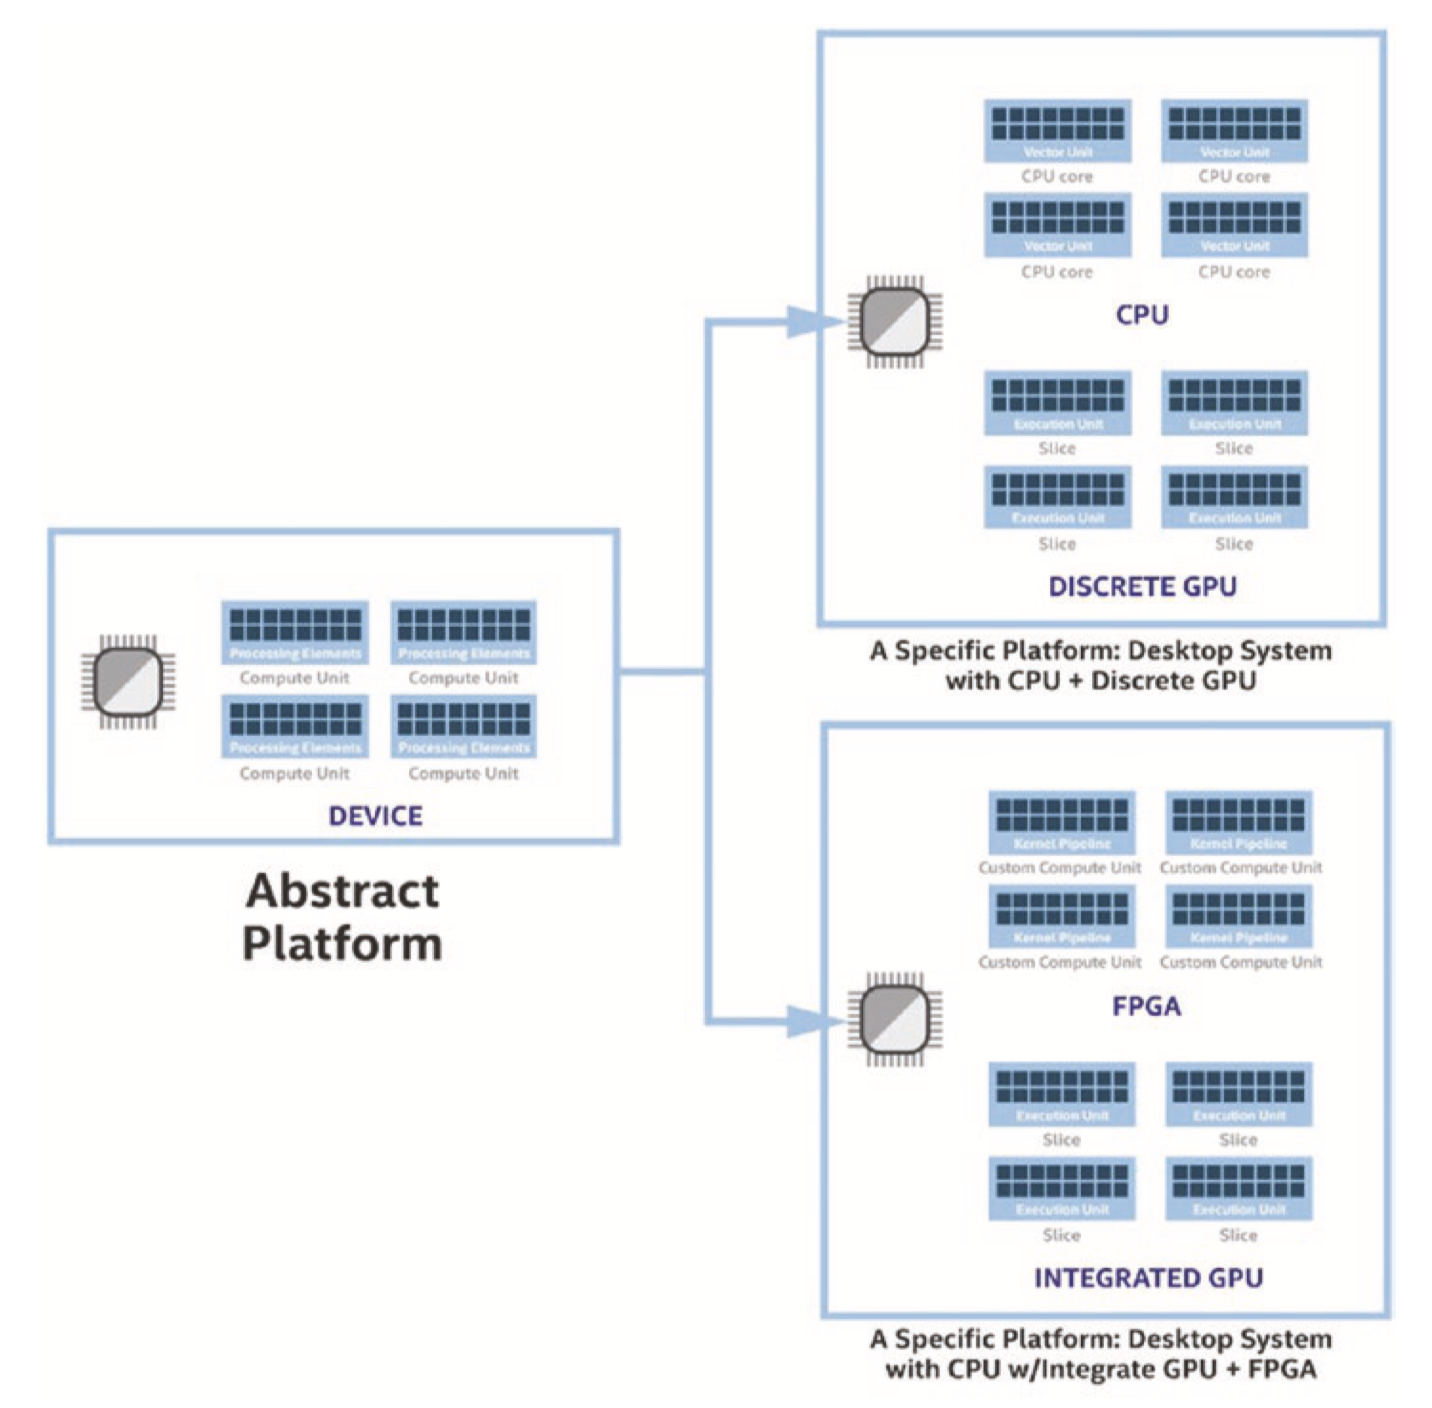
\includegraphics[width=0.9\textwidth]{figs/F13.1.png}
	\caption{\textit{基数排序示例。}}
\end{figure}

图 13.1 显示了如何使用 1 位基数通过基数排序对 4 位整数列表进行排序的示例。 
由于密钥为 4 位长,每次迭代处理 $1 \mathrm{bit}$,因此总共需要四次迭代。 在第一次迭代中,考虑最低有效位 (LSB)。 
迭代输入列表中LSB为0的所有键都放置在迭代输出列表的左侧,形成0位的桶。 
类似地,迭代输入列表中 LSB 为 1 的所有键都放置在迭代输出列表的右侧,形成 1 位的存储桶。 
请注意,在输出列表中的每个存储桶中,键的顺序均与输入列表中的顺序保持一致。 
换句话说,放置在同一存储桶中的键(即具有相同的 LSB)必须以与输入列表中相同的顺序出现在输出列表中。 
当我们讨论下一次迭代时,我们将看到为什么这种稳定性要求很重要。

在图 13.1 的第二次迭代中,第一次迭代的输出列表成为新的输入列表,并且考虑每个键的第二个 LSB。 
与第一次迭代一样,密钥被分为两个桶:一个桶用于存储第二个 LSB 为 0 的密钥,另一个桶用于存储第二个 LSB 为 1 的密钥。

由于保留了先前迭代的顺序,因此我们观察到第二次迭代的输出列表中的键现在按低两位排序。 
换句话说,所有低两位为 00 的密钥在前,其次是低两位为 01 的密钥,最后是低两位为 10 的密钥,最后是低两位为 11 的密钥。

在图 13.1 的第三次迭代中,在考虑密钥中的第三位的同时重复相同的过程。 
同样,由于保留了先前迭代的顺序,因此第三次迭代的输出列表中的键按低三位排序。 
最后,在第四次也是最后一次迭代中,在考虑第四位或最高有效位的同时重复相同的过程。 
在此迭代结束时,最终输出列表中的键按所有四位排序。

\subsection{并行基数排序}
基数排序中的每次迭代都取决于前一次迭代的整个结果。 因此,迭代是相对于彼此顺序执行的。 
每次迭代中都会出现并行基数排序的机会。 在本章的其余部分中,我们将重点关注单个基数排序迭代的并行化,
并理解迭代将一个接一个地执行。 换句话说,我们将重点关注执行单个基数排序迭代的内核的实现,
并假设主机代码为每次迭代调用该内核一次。

\begin{figure}[H]
	\centering
	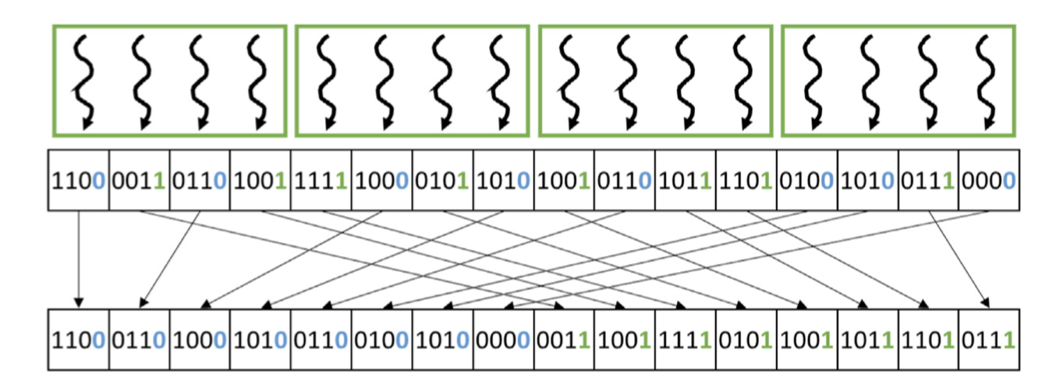
\includegraphics[width=0.9\textwidth]{figs/F13.2.png}
	\caption{\textit{通过为每个线程分配一个输入键来并行基数排序迭代。}}
\end{figure}

在 GPU 上并行化基数排序迭代的一种直接方法是让每个线程负责输入列表中的一个键。 
线程必须识别输出列表中键的位置,然后将键存储到该位置。 图 13.2 说明了应用于图 13.1 中第一次迭代的并行化方法。 
图13.2中的线程被图示为弯曲箭头,并且线程块被图示为箭头周围的框。 每个线程负责输入列表中位于其下方的键。 
在此示例中,16 个键由具有四个线程块的网格处理,每个线程块具有四个线程。 
实际上,每个线程块可能最多有1024个线程,输入量更大,导致线程块更多。 然而,我们在每个块中使用了少量线程来简化说明。

当每个线程分配给输入列表中的一个键时,每个线程仍然面临着识别其键在输出列表中的目标索引的挑战。 
识别该键的目标索引取决于该键映射到0桶还是1桶。 对于映射到 0 桶的键,可以通过以下方式找到目标索引:

\begin{figure}[H]
	\centering
	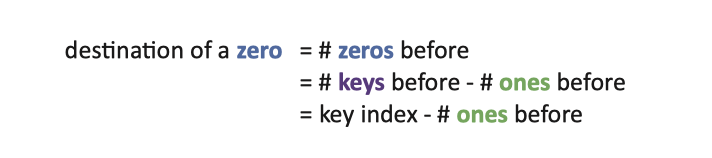
\includegraphics[width=0.9\textwidth]{figs/F13-a1.png}
\end{figure}

映射到 0 存储桶的键的目标索引(即 0 的目标)等于该键之前也映射到 0 存储桶的键的数量(即之前的 \# 个零)。 
由于所有键都映射到 0 桶或 1 桶,因此映射到 0 桶的键之前的键数
等于该键之前的键总数(即之前的 \# 个键)减去之前的键数 映射到第 1 个存储桶的键(即之前的 \# 个)。 
该键之前的键总数就是该键在输入列表中的索引(即键索引),这是很容易获得的。 
因此,查找映射到 0 存储桶的键的目标索引的唯一重要部分是计算其之前映射到 1 存储桶的键的数量。 
这个操作可以通过使用独占扫描来完成,我们很快就会看到。

对于映射到 0 桶的键,可以通过以下方式找到目标索引:

\begin{figure}[H]
	\centering
	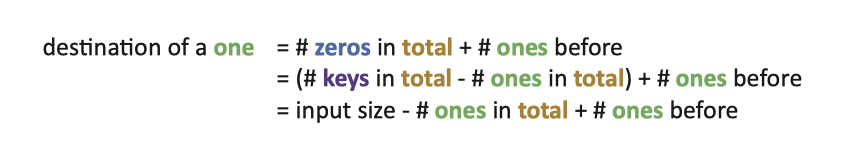
\includegraphics[width=0.9\textwidth]{figs/F13-a2.png}
\end{figure}

在输出数组中,映射到 0 存储桶的所有键必须位于映射到 1 存储桶的键之前。 
因此,映射到 1 存储桶的键的目标索引(即 1 的目标)等于映射到 0 存储桶的键总数(即总共 \# 个零)加上键的数量 在映射到第 1 个存储桶的键之前(即之前的 \# 个)。 
由于所有键都映射到 0 存储桶或 1 存储桶,
因此映射到 0 存储桶的键总数等于输入列表中的键总数(即总共 \# 个键)减去键总数 映射到 1 个存储桶(即总共 \# 个)。 
输入列表中的键总数就是输入大小,这是很容易获得的。 
因此,查找映射到 1 存储桶的键的目标索引的重要部分是计算其之前映射到 1 存储桶的键的数量,这与 0 存储桶情况所需的信息相同。 
同样,这个操作可以通过使用独占扫描来完成,我们很快就会看到。 映射到第 1 个存储桶的键总数可以作为独占扫描的副产品找到。

\begin{figure}[H]
	\centering
	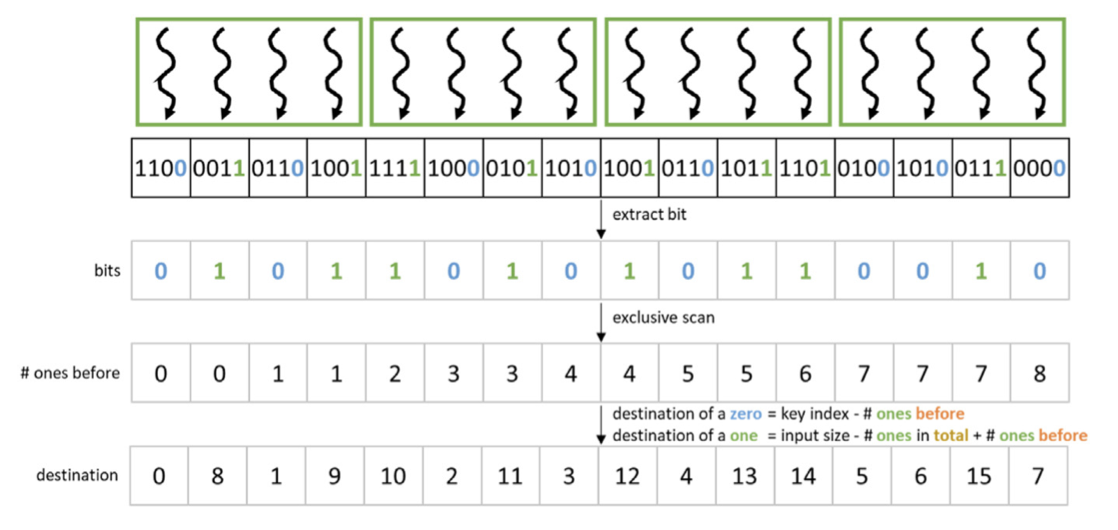
\includegraphics[width=0.9\textwidth]{figs/F13.3.png}
	\caption{\textit{查找每个输入键的目的地。}}
\end{figure}

图 13.3 显示了图 13.2 示例中每个线程为查找其键的目标索引而执行的操作。 
执行这些操作的相应内核代码如图 13.4 所示。 首先,每个线程识别其负责的键的索引(第 03 行),执行边界检查(第 04 行),
并从输入列表加载键(第 06 行)。 接下来,每个线程从密钥中提取当前迭代的位,以确定它是 0 还是 1(第 07 行)。

这里,迭代次数 iter 告诉我们感兴趣的位的位置。 通过将键向右移动这个量,我们将位移动到最右边的位置。 
通过在移位键和 1 之间应用按位与运算 (\&),我们将移位键中除最右边位之外的所有位清零。 
因此,位的值将是我们感兴趣的位的值。 在图 13.3 的示例中,由于该示例针对迭代 0,因此提取了 LSB,如标记位的行所示。

一旦每个线程从密钥中提取了它感兴趣的位,它就会将该位存储到内存中(第 08 行),
并且线程协作对这些位执行独占扫描(第 10 行)。 我们在第 11 章“前缀和(扫描)”中讨论了如何执行独占扫描。 
对独占扫描的调用是在边界检查之外执行的,因为线程可能需要在进程中执行屏障同步,因此我们需要确保所有线程都处于活动状态。 
为了在网格中的所有线程之间进行同步,我们假设可以使用类似于第 11 章“前缀和(扫描)”中讨论的单遍扫描中使用的复杂技术。 
或者,我们可以终止内核,从主机调用另一个内核来执行扫描,然后调用第三个内核来执行扫描后的操作。 
在这种情况下,每次迭代都需要启动三次网格,而不是一次。 独占扫描操作产生的数组在每个位置包含该位置之前的位的总和。 
由于这些位要么是 0 要么是 1 ,因此该位置之前的位之和等于该位置之前的 1 的数量(即映射到 1 存储桶的键的数量)。 
在图 13.3 的示例中,独占扫描的结果显示在前面标有 \# those 的行中。 
每个线程访问该数组以获取其位置之前 1 的数量(第 12 行)以及输入列表中 1 的总数(第 13 行)。 
然后,每个线程可以使用我们之前导出的表达式(第 14-15 行)来识别其键的目的地。 
识别出其目标索引后,线程可以继续将其负责的键存储在输出列表中的相应位置(第 16 行)。 
在图 13.3 的示例中,目标索引显示在标记为目标的行中。 读者可以参考图13.2来验证所获得的值确实是每个元素的正确目标索引。

\subsection{优化内存合并}
我们刚刚描述的方法对于并行基数排序迭代非常有效。 
然而,这种方法效率低下的一个主要根源是对输出列表的写入表现出无法充分合并的访问模式。 
考虑图 13.2 中的每个线程如何将其密钥写入输出列表。 
在第一个线程块中,第一个线程写入0桶,第二个线程写入1桶,第三个线程写入0桶,第四个线程写入1桶。 
因此,具有连续索引值的线程不一定会写入连续的内存位置,从而导致合并效果不佳并需要为每个 warp 发出多个内存请求。

\begin{figure}[H]
	\centering
	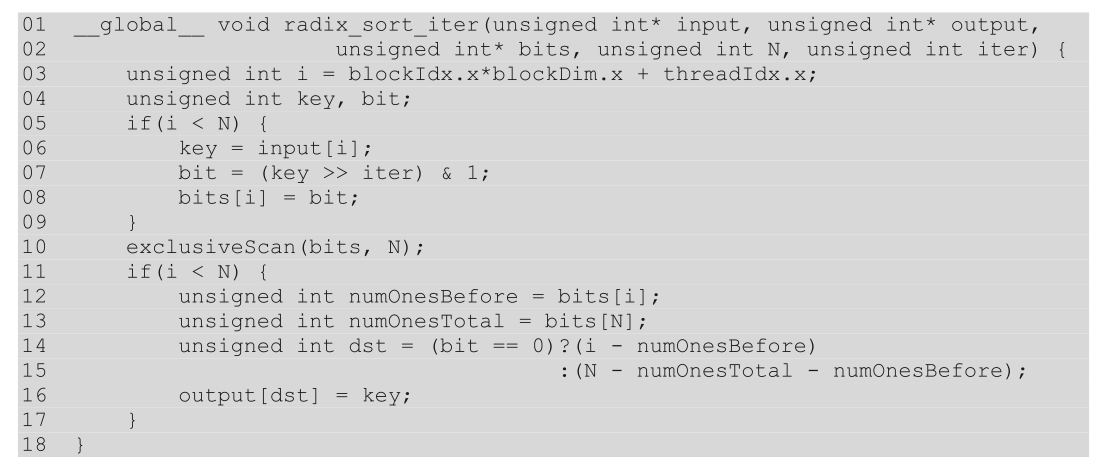
\includegraphics[width=0.9\textwidth]{figs/F13.4.png}
	\caption{\textit{基数排序迭代内核代码。}}
\end{figure}

回想一下第 6 章“性能注意事项”,有多种方法可以在内核中实现更好的内存合并:(1) 重新排列线程,(2) 重新排列线程访问的数据,
或 (3) 在共享内存上执行不可合并的访问 以合并的方式在共享内存和全局内存之间传输数据。 
为了优化本章中的合并,我们将使用第三种方法。 我们将让每个线程块在共享内存中维护自己的局部存储桶,
而不是让所有线程以未合并的方式将其密钥写入全局内存存储桶。 也就是说,我们将不再执行如图 13.4 所示的全局排序。 
相反,每个块中的线程将首先执行块级局部排序,以分离共享内存中映射到 0 存储桶的键和映射到 1 存储桶的键。 
之后,桶将以合并的方式从共享内存写入全局内存。

\begin{figure}[H]
	\centering
	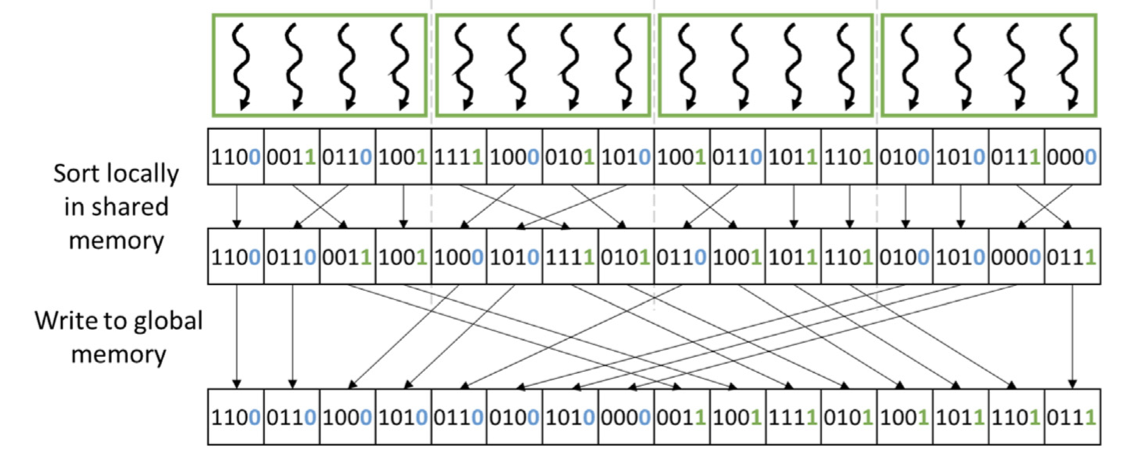
\includegraphics[width=0.9\textwidth]{figs/F13.5.png}
	\caption{\textit{在排序到全局内存中之前,通过在共享内存中进行本地排序来优化内存合并。}}
\end{figure}

图 13.5 显示了如何增强图 13.2 中示例的内存合并的示例。 
在此示例中,每个线程块首先对其拥有的键执行局部基数排序,并将输出列表存储到共享内存中。 
局部排序可以按照与之前进行全局排序相同的方式来完成,并且要求每个线程块仅执行局部独占扫描,而不需要全局扫描。 
在局部排序之后,每个线程块以更加合并的方式将其局部存储桶写入全局存储桶。 
例如,在图 13.5 中,考虑第一个线程块如何将其存储桶写入全局内存。 
前两个线程在写入 0 桶时都写入全局内存中的相邻位置,而后两个线程在写入 1 桶时也写入全局内存中的相邻位置。 
因此,对全局内存的大部分写入将被合并。

此优化的主要挑战是每个线程块识别其每个局部存储桶在相应全局存储桶中的开始位置。 
线程块的局部存储桶的开始位置取决于其他线程块中的局部存储桶的大小。 
具体地,一个线程块的局部0桶的位置位于前面线程块的所有局部0桶之后。 
另一方面,线程块的局部1桶的位置位于所有线程块的所有局部0桶以及之前线程块的所有局部1桶之后。 
这些位置可以通过对线程块的局部存储桶大小执行独占扫描来获得。

\begin{figure}[H]
	\centering
	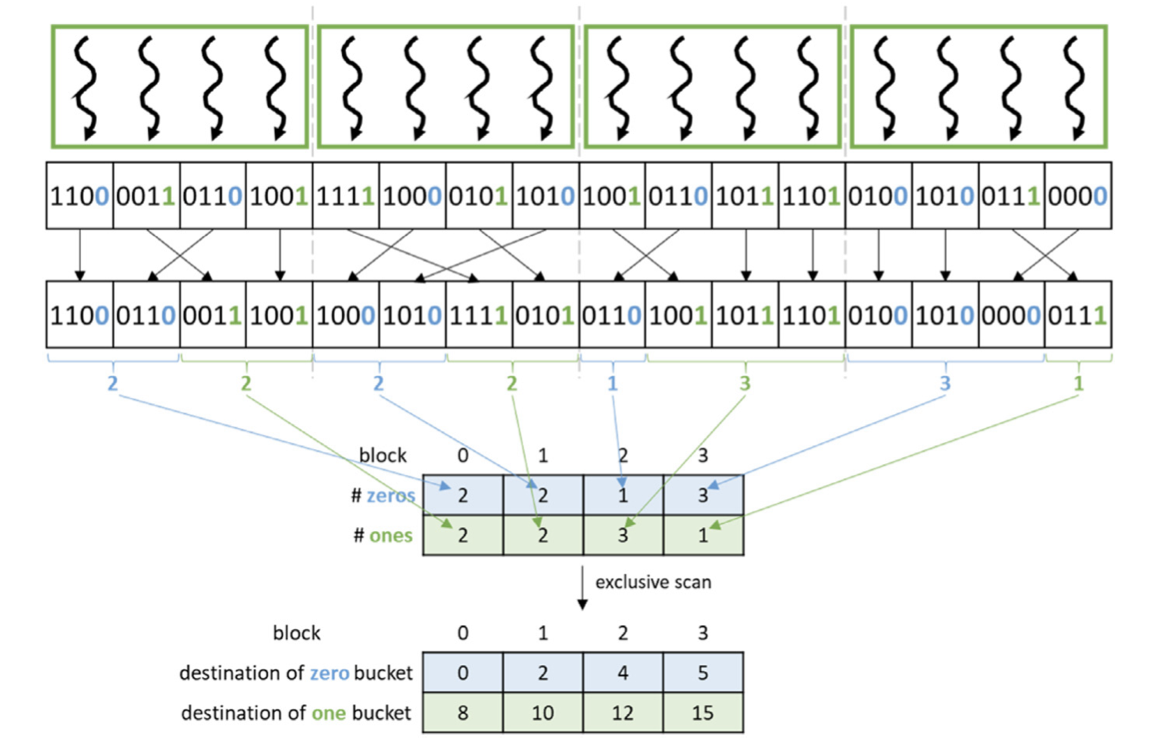
\includegraphics[width=0.9\textwidth]{figs/F13.6.png}
	\caption{\textit{查找每个线程块的本地存储桶的目的地。}}
\end{figure}

图 13.6 显示了如何使用独占扫描来查找每个线程块的局部存储桶的位置的示例。 
完成局部基数排序后,每个线程块识别其每个局部桶中的键的数量。 接下来,每个线程块将这些值存储在表中,如图 13.6 所示。 
该表按行优先顺序存储,这意味着它连续放置所有线程块的局部 0 存储桶的大小,然后是局部 1 存储桶的大小。 
表构建完成后,将对线性化表执行独占扫描。 结果表由每个线程块的局部存储桶的起始位置组成,这就是我们要查找的值。

一旦线程块识别出其局部存储桶在全局内存中的开始位置,该块中的线程就可以继续将其密钥从局部存储桶存储到全局存储桶。 
为此,每个线程需要跟踪 0 存储桶与 1 存储桶中键的数量。 在写入阶段,每个块中的线程将根据其线程索引值在任一存储桶中写入键。 
例如,对于图13.6中的块2,线程0将单个密钥写入0存储桶中,线程$1-3$将三个密钥写入1存储桶中。 
相比之下,对于图13.6中的块3,线程0-2将三个键写入0桶中,线程3将1键写入1桶中。 
因此每个线程需要测试它是否负责在局部0桶或1桶中写入密钥。 
每个块都会跟踪其两个局部存储桶中的每个存储桶中的键数,
以便线程可以确定其 threadIdx 值落在何处并参与 0 存储桶键或 1 存储桶键的写入。 我们将这种优化的实现留给读者作为练习。

\subsection{基值的选择}
到目前为止,我们已经以 1 位基数为例了解了如何并行化基数排序。 
对于示例中的 4 位键,需要四次迭代(每位迭代一次)才能对键进行完全排序。 
一般来说,对于 $N$ 位的键,需要 $N$ 迭代才能对键进行完全排序。 为了减少所需的迭代次数,可以使用更大的基值。

\begin{figure}[H]
	\centering
	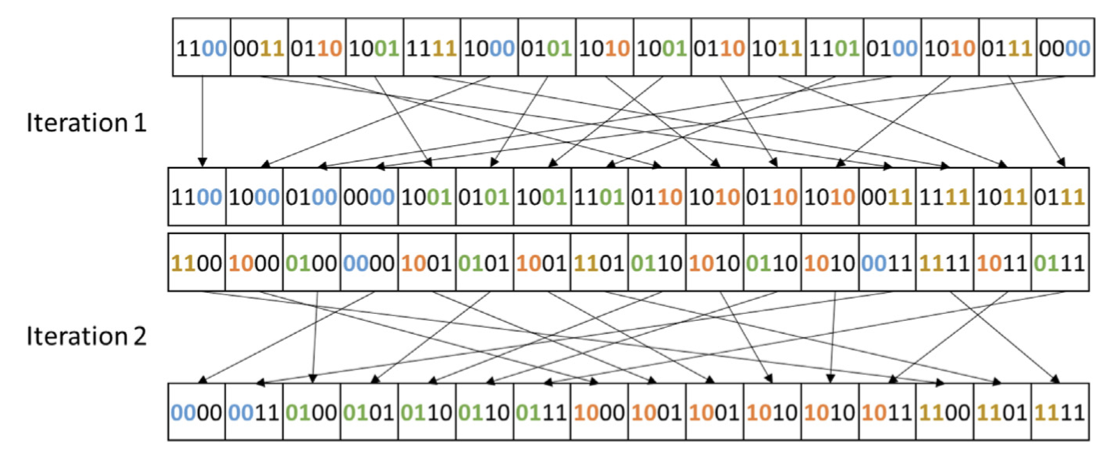
\includegraphics[width=0.9\textwidth]{figs/F13.7.png}
	\caption{\textit{使用 2 位基数的基数排序示例。}}
\end{figure}

图 13.7 显示了如何使用 2 位基数执行基数排序的示例。 每次迭代使用两位将密钥分配到桶中。 
因此,仅使用两次迭代即可对 4 位密钥进行完全排序。 在第一次迭代中,考虑较低的两位。 
键分布在四个存储桶中,对应的键的低两位是 $00,01,10$ 和 11 。 在第二次迭代中,考虑高两位。 
然后根据高两位将密钥分配到四个存储桶中。 与 1 位示例类似,每个存储桶中键的顺序均从上一次迭代中保留。 
保留每个存储桶内键的顺序可确保在第二次迭代后键按所有四位完全排序。

\begin{figure}[H]
	\centering
	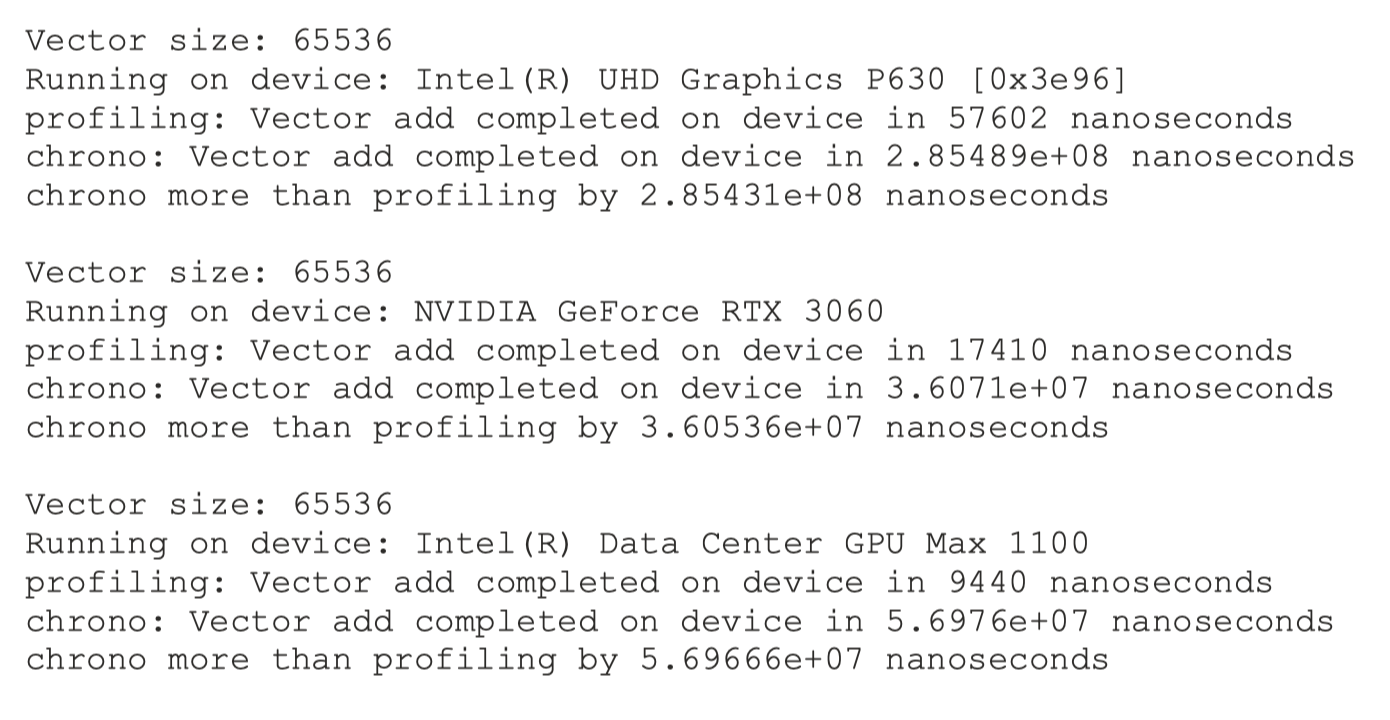
\includegraphics[width=0.9\textwidth]{figs/F13.8.png}
	\caption{\textit{并行基数排序迭代并使用 2 位基数的共享内存优化内存合并。}}
\end{figure}

与 1 位示例类似,可以通过为输入列表中的每个键分配一个线程以查找键的目标索引并将其存储在输出列表中来并行化每次迭代。 
为了优化内存合并,每个线程块可以在共享内存中局部对其键进行排序,然后以合并的方式将局部存储桶写入全局内存。 
图 13.8 显示了如何并行化基数排序迭代并使用共享内存优化内存合并的示例。

1 位示例和 2 位示例之间的主要区别在于如何将密钥分成四个存储桶而不是两个存储桶。 
对于每个线程块内的局部排序,通过应用两个连续的 1 位基数排序迭代来执行 2 位基数排序。 
这些 1 位迭代中的每一个都需要其自己的独占扫描操作。 
然而,这些操作是线程块局部的,因此在两个 1 位迭代之间不存在跨线程块的协调。 
一般来说,对于 $r$ 位基数,需要 $r$ 局部 1 位迭代来将键排序到 $2^{r}$ 局部存储桶中。

\begin{figure}[H]
	\centering
	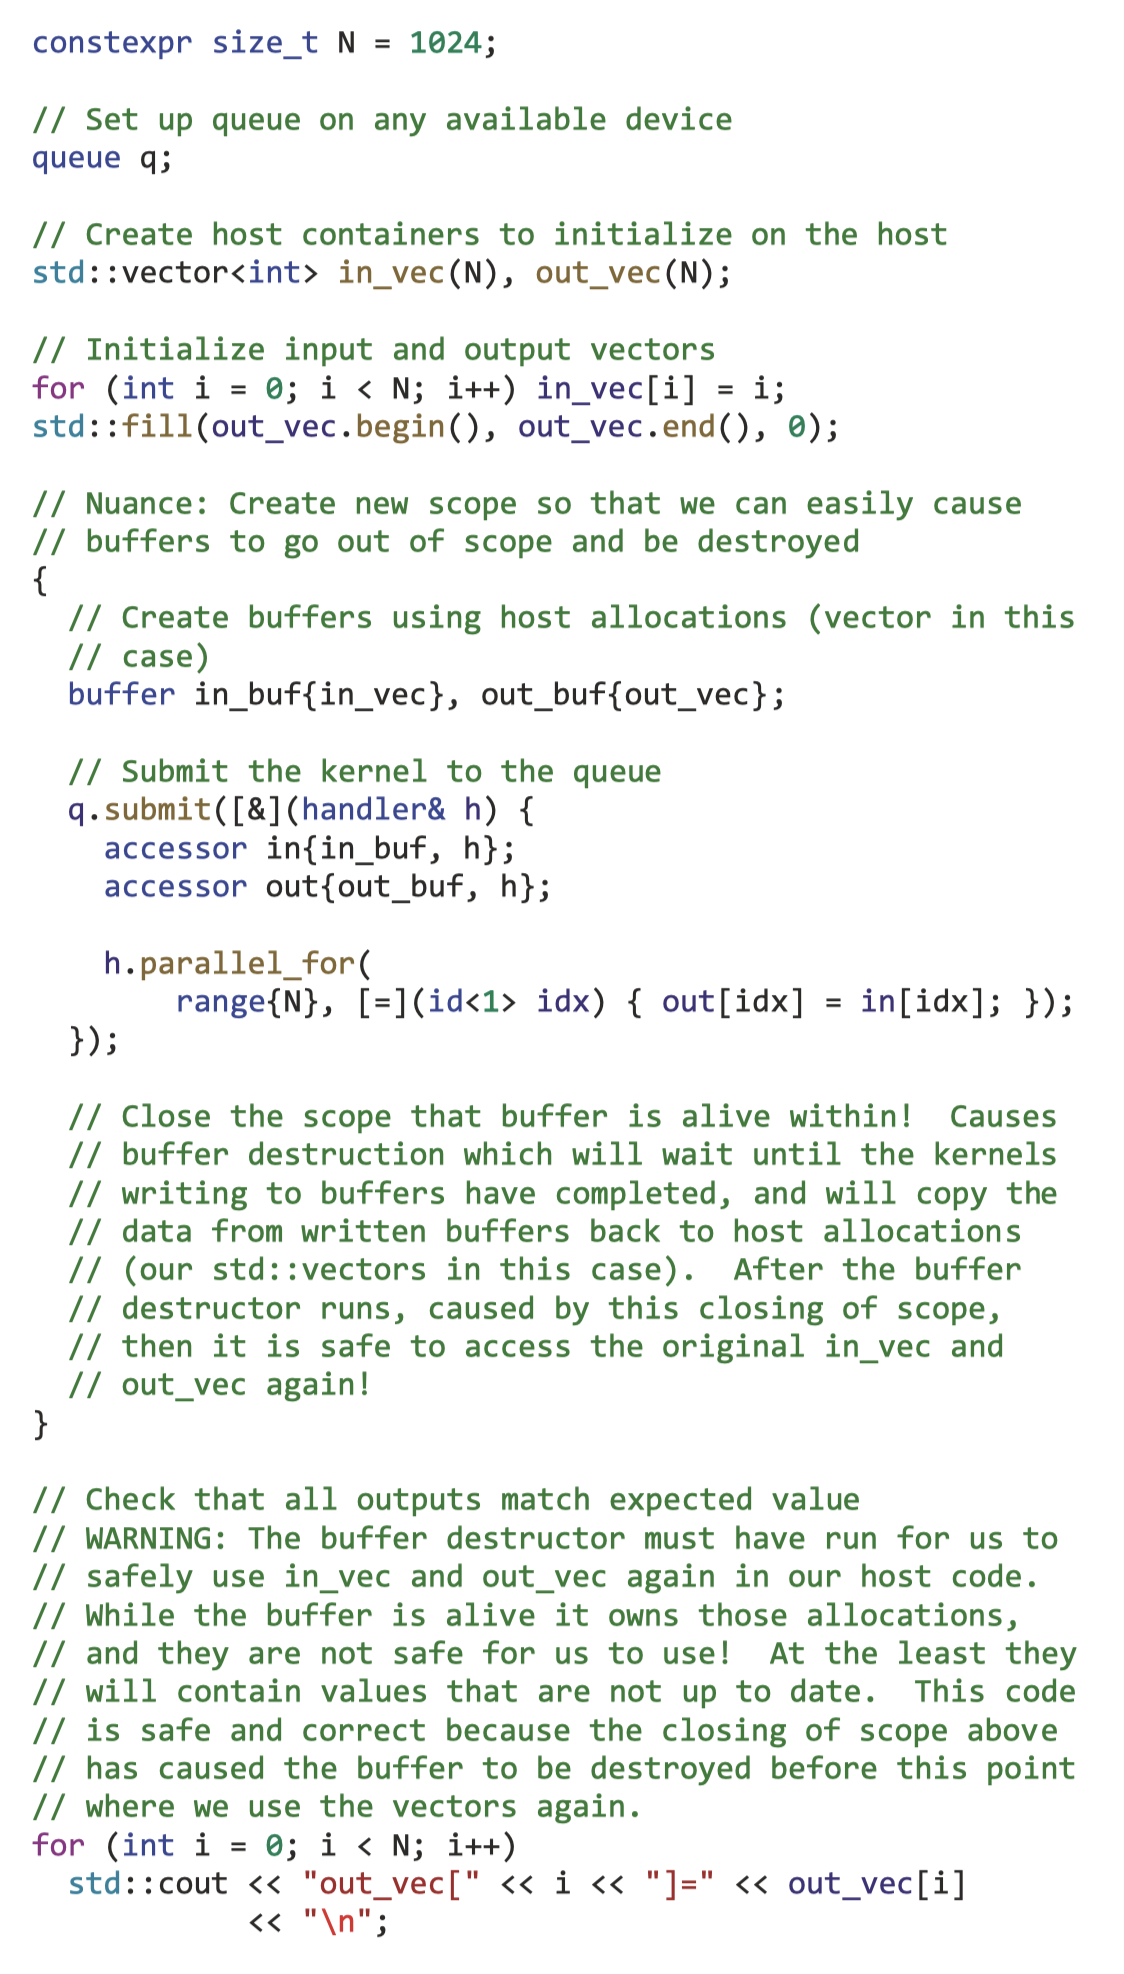
\includegraphics[width=0.9\textwidth]{figs/F13.9.png}
	\caption{\textit{查找 2 位基数的每个块的本地存储桶的目的地。}}
\end{figure}

局部排序完成后,每个线程块必须在全局输出列表中找到其每个局部桶的位置。 
图 13.9 显示了如何针对 2 位基数示例找到每个局部存储桶的目的地的示例。 该过程类似于图 13.6 中的 1 位示例。 
每个线程块将每个局部桶中的键数量存储到一个表中,然后扫描该表以获得每个局部桶的全局位置。 
与 1 位基数示例的主要区别在于,每个线程块有四个局部存储桶,而不是两个,因此独占扫描操作是在具有四行而不是两行的表上执行的。 
一般来说,对于 $r$ 位基数,独占扫描操作是在具有 $2^{r}$ 行的表上执行的。

我们已经看到,使用较大基数的优点是它减少了对键进行完全排序所需的迭代次数。 
更少的迭代意味着更少的网格启动、全局内存访问和全局独占扫描操作。 然而,使用较大的基数也有缺点。 
第一个缺点是每个线程块有更多的局部存储桶,而每个存储桶的键更少。 
因此,每个线程块需要写入更多不同的全局内存桶部分,并且需要写入每个部分的数据更少。 
因此,随着基数变大,内存合并的机会就会减少。 第二个缺点是,应用全局独占扫描的表会随着基数的增大而变大。 
因此,全局独占扫描的开销随着基数的增加而增加。 因此基数不能任意大。 
基值的选择必须在迭代次数和内存合并行为以及全局独占扫描的开销之间取得平衡。 我们将使用多位基数实现基数排序作为读者的练习。

\subsection{线程粗化以改善合并}
跨多个线程块并行基数排序的代价是对全局内存的写入合并不佳。 每个线程块都有自己的局部存储桶,并将其写入全局内存。 
拥有更多的线程块意味着每个线程块拥有更少的键,这意味着局部存储桶会更小,当它们写入全局内存时暴露的合并机会更少。 
如果这些线程块要并行执行,那么不良合并的代价可能是值得的。 然而,如果这些线程块要被硬件串行化,就会付出不必要的代价。

\begin{figure}[H]
	\centering
	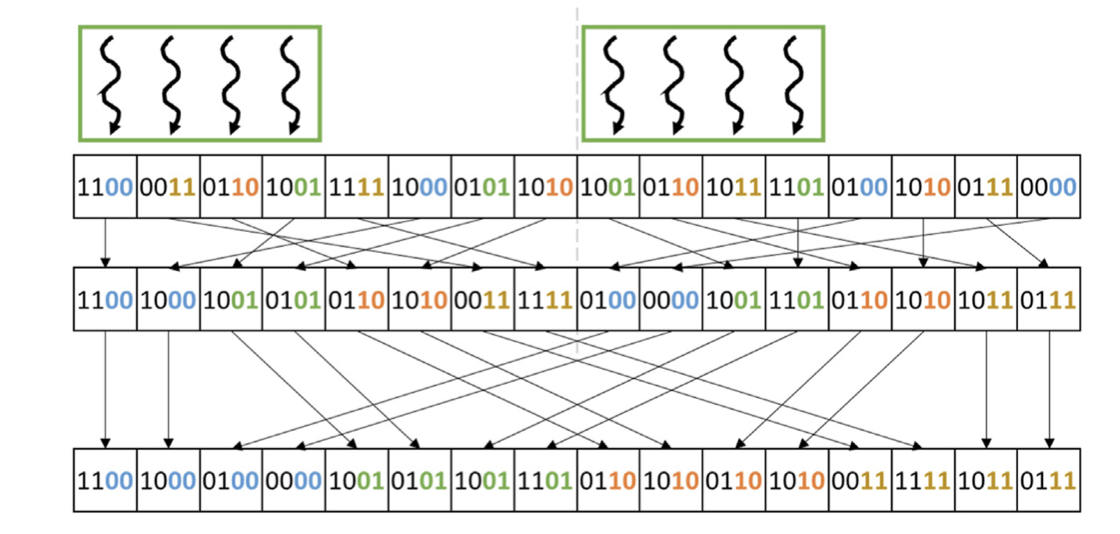
\includegraphics[width=0.9\textwidth]{figs/F13.10.png}
	\caption{\textit{对 2 位基数进行基数排序,并通过线程粗化来改进内存合并。}}
\end{figure}

为了解决这个问题,可以应用线程粗化,将每个线程分配给输入列表中的多个键,而不是仅一个。 
图 13.10 说明了如何将线程粗化应用于 2 位基数示例的基数排序迭代。 
在这种情况下,每个线程块比图 13.8 中的示例负责更多的键。 因此,每个线程块的局部存储桶更大,从而提供更多合并机会。 
当我们比较图 13.8 和图 13.10 时,很明显,在图 13.10 中,更可能是连续线程写入连续内存位置的情况。

跨多个线程块并行化基数排序的另一个代价是执行全局独占扫描以识别每个线程块的局部存储桶的目的地的开销。 
回想一下图 13.9,执行独占扫描的表的大小与桶的数量以及块的数量成正比。 
通过应用线程粗化,减少了块的数量,从而减少了表的大小和独占扫描操作的开销。 我们将线程粗化在基数排序中的应用作为读者的练习。

\subsection{并行归并排序}
当键要按字典顺序排序时,基数排序适用。 
然而,如果要根据复杂比较运算符定义的复杂顺序对键进行排序,那么基数排序就不适合,并且需要基于比较的排序算法。 
此外,通过简单地改变比较运算符,基于比较的排序算法的实现可以更容易地适应不同类型的键。 
相反,使基于非比较的排序算法(例如基数排序)的实现适应不同类型的键可能涉及创建不同版本的实现。 
这些考虑因素可能会使基于比较的排序在某些情况下更有利,尽管它们的复杂性更高。

一种适合并行化的基于比较的排序是合并排序。 
合并排序的工作原理是将输入列表划分为段,对每个段进行排序(使用合并排序或其他排序算法),然后对已排序的段执行有序合并。

\begin{figure}[H]
	\centering
	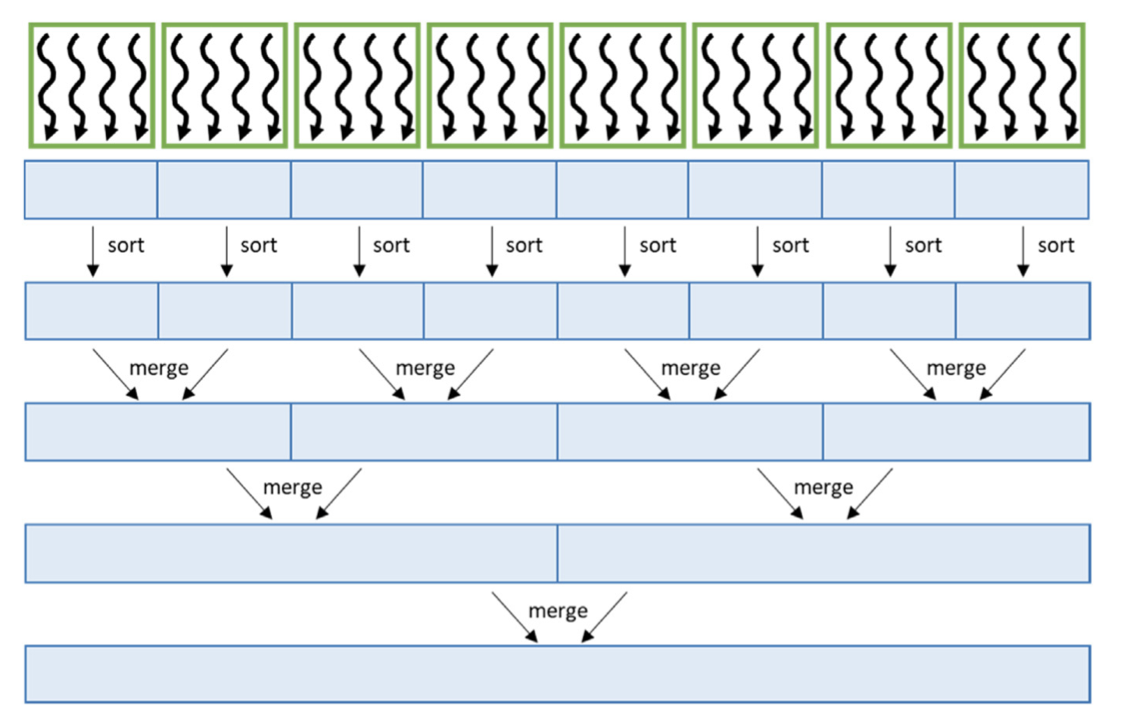
\includegraphics[width=0.9\textwidth]{figs/F13.11.png}
	\caption{\textit{并行合并排序。}}
\end{figure}

图 13.11 显示了如何并行化合并排序的示例。 最初,输入列表被分为许多段,每个段都使用某种有效的排序算法独立排序。 
之后,每对段都合并为一个段。 重复此过程,直到所有键都成为同一段的一部分。

在每个阶段,可以通过并行执行不同的合并操作以及合并操作内的并行化来并行化计算。 
在早期阶段,有更多独立的合并操作可以并行执行。 
在后期阶段,独立的合并操作较少,但每个合并操作合并更多的键,从而在合并操作中暴露出更多的并行性。 
例如,在图 13.11 中,第一个合并阶段由四个独立的合并操作组成。 
因此,我们的八个线程块网格可以分配两个线程块来并行处理每个合并操作。 
在下一阶段,只有两次合并操作,但每次操作合并两倍数量的键。 
因此,我们的八个线程块网格可以分配四个线程块来并行处理每个合并操作。 我们在第 12 章“合并”中了解了如何并行化合并操作。 
我们将基于并行合并的合并排序的实现留给读者作为练习。

\subsection{其他并行排序方法}
上面概述的算法只是并行排序数据的多种可能方法中的两种。 在本节中,我们简要概述了读者可能感兴趣的一些其他方法。

最简单的并行排序方法之一是奇偶转置排序。 它首先并行比较每对偶数/奇数键,
即从第一个偶数索引开始具有索引 $\mathrm{k}$ 和 $\mathrm{k}+1$ 的键。 
如果位置 $\mathrm{k}+1$ 处的键小于位置 $\mathrm{k}$ 处的键,则交换键的位置。 
然后对每个奇/偶对键重复此步骤,即从第一个奇数索引开始具有索引 $\mathrm{k}$ 和 $\mathrm{k}+1$ 的键。 
重复这些交替阶段,直到两个阶段都完成且无需交换密钥。 
奇偶转置排序与顺序冒泡排序算法非常相似,并且与冒泡排序一样,
它在大型序列上效率较低,因为它可能会执行 N 序列的 $O\left(N^{2}\right)$ 工作  元素。

转置排序使用固定的比较模式,并在元素无序时交换元素。 它很容易并行化,因为每个步骤都会比较不重叠的键对。 
有一整类排序方法使用固定的比较模式来对序列进行排序,通常是并行的。 
这些方法通常称为排序网络,最著名的并行排序网络是 Batcher 的双调排序和奇偶合并排序(Batcher,1968)。 
Batcher 的算法对固定长度的序列进行操作,比奇偶转置排序更高效,
只需对 $\mathrm{N O}\left(N \cdot \log^{2} N\right)$ 的序列进行比较 元素。 
尽管这些算法的成本渐进地比合并排序等方法的 $O(N \cdot \log N) \cos t$ 更差,
但实际上,由于其简单性,它们通常是小序列上最有效的方法 。

大多数不使用排序网络典型的固定比较集的基于比较的并行排序可以分为两大类。 
第一个将未排序的输入划分为图块,对每个图块进行排序,然后执行大部分工作来组合这些图块以形成输出。 
我们在本章中描述的合并排序就是这种算法的一个例子; 大部分工作是在组合排序图块的合并树中执行的。 
第二类的大部分工作集中在对未排序的序列进行分区上,这样组合分区就相对简单了。 
样本排序算法(Frazer 和 McKellar,1970)是此类的典型例子。 
示例排序首先从输入中选择 $\mathrm{p}-1$ 键(例如随机),对它们进行排序,
然后使用它们将输入分区到 $\mathrm{p}$ 存储桶中,
以便所有键都在 存储桶 $\mathrm{k}$ 大于任何存储桶 $\mathrm{j}<\mathrm{k}$ 中的所有键,
并且小于任何存储桶 $\mathrm{j}>\mathrm{k}$ 中的所有键。 此步骤类似于快速排序执行的双向划分的 p 路推广。 
以这种方式对数据进行分区后,每个桶都可以独立排序,并且排序的输出只需按顺序连接桶即可形成。 
对于超大型序列,样本排序算法通常是最有效的选择,其中数据必须分布在多个物理内存中,包括单个节点中多个 GPU 的内存中。 
在实践中,对键进行过采样很常见,因为适度的过采样将导致高概率的平衡分区(Blelloch 等人,1991)。

正如合并排序和样本排序代表了基于比较的排序的自下而上和自上而下的策略一样,
基数排序算法也可以设计为遵循自下而上或自上而下的策略。 我们在本章中描述的基数排序更完整地描述为 LSB,或者更一般地说,
最低有效数字 (LSD) 基数排序。 该算法的后续步骤从密钥的 LSD 开始,一直到最高有效数字 (MSD)。 
MSD 基数排序采用相反的策略。 首先使用 MSD 将输入划分到与该数字的可能值相对应的存储桶中。 
然后使用下一个 MSD 在每个存储桶中独立应用相同的分区。 到达 LSD 后,整个序列将被排序。 
与样本排序一样,MSD 基数排序通常是非常大的序列的更好选择。 
LSD 基数排序需要在每个步骤中对数据进行全局改组,而 MSD 基数排序的每个步骤都对数据的逐渐更局部的区域进行操作。

\subsection{总结}
在本章中,我们了解了如何在 GPU 上并行对键(及其关联值)进行排序。 
在本章的大部分内容中,我们关注基数排序,它通过将键分布在存储桶中来对键进行排序。 
对密钥中的每个数字重复分配过程,同时保留前一个数字迭代的顺序,以确保密钥根据末尾的所有数字进行排序。 
每次迭代都是通过为输入列表中的每个键分配一个线程并让该线程查找输出列表中键的目的地来并行化的,
这涉及与其他线程协作来执行独占扫描操作。

优化基数排序的关键挑战之一是在将键写入输出列表时实现合并内存访问。 
增强合并的一个重要优化是让每个线程块对共享内存中的局部存储桶执行局部排序,然后以合并的方式将每个局部存储桶写入全局内存。 
另一种优化是增加基数的大小,以减少所需的迭代次数,从而减少启动的网格数量。 
但是,基数大小不应增加太多,因为这会导致较差的合并以及全局独占扫描操作的更多开销。 
最后,应用线程粗化可以有效地改善内存合并以及减少全局独占扫描的开销。

基数排序的优点是计算复杂度低于 O(Nlog(N))。 但是,基数排序仅适用于有限类型的键,例如整数。 
因此,我们还研究了适用于一般类型键的基于比较的排序的并行化。 一类适合并行化的基于比较的排序算法是合并排序。 
合并排序可以通过并行执行不同输入段的独立合并操作以及在每个合并操作内并行化来并行化,正如我们在第 12 章“合并”中看到的那样。

在 GPU 上实现和优化并行排序算法的过程很复杂,普通用户更有可能使用 GPU 并行排序库,
例如 Thrust(Bell 和 Hoberock,2012),而不是从头开始实现自己的排序内核 。 
尽管如此,并行排序仍然是优化并行模式的权衡的一个有趣的案例研究。